\part{Informatik 2 - Sommersemester 2009}
\chapter{Grundlagen Informatik}
\section{29.04.2009}
\subsection{GI-29.04.2009-IMG-1}
\begin{tikzpicture}[->,>=stealth',shorten >=1pt,auto,node distance=2.8cm,semithick]
\node (n0) {$q_0$};
\node (n1) [right of=n0] {$q'$};
\node (n2) [right of=n1] {$q''$};
\node (n3) [right of=n2] {$p_{i_1}$};

\path[->] (n0) edge node[above] {$\epsilon$} (n1);
\path[->] (n1) edge node[above] {$a$} (n2);
\path[->] (n2) edge node[above] {$\epsilon$} (n3);
\path[->] (n0) edge[bend left] node[above] {$a$} (n3);
\end{tikzpicture}
\Img{GI-29.04.2009-IMG-1}

\subsection{GI-29.04.2009-IMG-2}
\begin{tikzpicture}[->,>=stealth',shorten >=1pt,auto,node distance=2.8cm,semithick]
\node[state, initial, initial text=, accepting] (n0) {$\overline{0}$};
\node[state] (n1) [right of=n0] {$\overline{1}$};
\node[state] (n2) [right of=n1] {$\overline{2}$};
\node [left of=n0, node distance=1.5cm] {$M_1$:};

\path[->] (n0) edge[loop above] node[right] {$0$} ();
\path[->] (n2) edge[loop above] node[right] {$1$} ();

\path[->] (n0) edge[bend left] node[above] {$1$} (n1);
\path[->] (n1) edge[bend left] node[below] {$1$} (n0);
\path[->] (n1) edge[bend left] node[above] {$0$} (n2);
\path[->] (n2) edge[bend left] node[below] {$0$} (n1);
\end{tikzpicture}
\Img{GI-29.04.2009-IMG-2.1}

\begin{tikzpicture}[->,>=stealth',shorten >=1pt,auto,node distance=2.8cm,semithick]
\node[state, initial, initial text=] (n0) {$\epsilon$};
\node[state] (n1) [right of=n0] {$1$};
\node[state] (n2) [right of=n1] {$11$};
\node[state, accepting] (n3) [right of=n2] {$111$};
\node [left of=n0, node distance=1.5cm] {$M_2$:};

\path[->] (n0) edge[loop above] node[right] {$0$} ();
\path[->] (n3) edge[loop above] node[right] {$0,1$} ();

\path[->] (n0) edge node[above] {$1$} (n1);
\path[->] (n1) edge node[above] {$1$} (n2);
\path[->] (n2) edge node[above] {$1$} (n3);

\path[->] (n1) edge[bend left] node[below] {$0$} (n0);
\path[->] (n2) edge[bend right] node[above] {$0$} (n0);
\end{tikzpicture}
\Img{Gi-29.04.2009-IMG-2.2}

\subsection{GI-29.04.2009-IMG-3}
\begin{tikzpicture}[->,>=stealth',shorten >=1pt,auto,node distance=2.8cm,semithick]
\node[state, initial, initial text=] (n0) {$\begin{array}{c}\overline{0}\\\epsilon\end{array}$};
\node[state] (n1) [right of=n0] {$\begin{array}{c}\overline{1}\\1\end{array}$};
\node[state] (n2) [right of=n1] {$\begin{array}{c}\overline{1}\\1\end{array}$};
\node[state] (n3) [right of=n2] {$\begin{array}{c}\overline{2}\\\epsilon\end{array}$};
\node[state] (n4) [below of=n1] {$\begin{array}{c}\overline{0}\\11\end{array}$};
\node[state] (n5) [below of=n2] {$\begin{array}{c}\overline{2}\\1\end{array}$};
\node (n6) [right of=n5] {$\dots$};
\node[state, accepting] (n7) [right of=n6] {$\begin{array}{c}\overline{0}\\111\end{array}$};
\node[left of=n0,node distance=2.0cm] {$M$:};

\path[->] (n0) edge[loop above] node[right] {$0$} ();

\path[->] (n0) edge node[above] {$1$} (n1);
\path[->] (n1) edge node[above] {$0$} (n2);
\path[->] (n2) edge node[above] {$0$} (n3);
\path[->] (n1) edge node[right] {$1$} (n4);
\path[->] (n2) edge node[right] {$1$} (n5);
\end{tikzpicture}
\Img{GI-29.04.2009-IMG-3}

\section{30.04.2009}
\subsection{IMG-30.04.2009-IMG-1}
\begin{tikzpicture}[->,>=stealth',shorten >=1pt,auto,node distance=2.8cm,semithick]
\node (n0) {$\epsilon$-NEA};
\node (n1) [right of=n0] {NEA};
\node (n2) [right of=n1] {DEA};

\path[->] (n0) edge[bend left] (n1);
\path[->] (n1) edge[bend left] (n2);
\path[->] (n0) edge[bend right] (n2);
\path[->] (n1) edge (n0);
\path[->] (n2) edge (n1);
\end{tikzpicture}
\Img{GI-30.04.2009-IMG-1}

\subsection{IMG-30.04.2009-IMG-2}
\begin{tikzpicture}[->,>=stealth',shorten >=1pt,auto,node distance=2.8cm,semithick]
\node[state, initial, initial text=] (n0) {$A$};
\node[state] (n1) [right of=n0] {$B$};
\node[state,accepting] (n2) [right of=n1] {$C$};
\node at (n2.east) [right,node distance=0.5cm] {$Q = \{A, B, C\}$};

\path[->] (n0) edge[loop above] node[right] {$1, 0$} ();
\path[->] (n0) edge node[above] {$0$} (n1);
\path[->] (n1) edge node[above] {$0$} (n2);
\end{tikzpicture}
\Img{GI-30.04.2009-IMG-2.1}

\begin{tikzpicture}[->,>=stealth',shorten >=1pt,auto,node distance=2.8cm,semithick]
\node[state, initial, initial text=] (n0) {$\{A\}$};
\node[state] (n1) [right of=n0] {$\{A, B\}$};
\node[state,accepting] (n2) [right of=n1] {$\{A, B, C\}$};
\node at (n2.east) [right,node distance=0.5cm] {$Q_P = \mathcal{P} (Q)$};

\path[->] (n0) edge[loop above] node[right] {$1, 0$} ();
\path[->] (n0) edge[loop below] node[right] {$0$} ();
\path[->] (n0) edge node[below] {$0$} (n1);
\path[->] (n1) edge node[above] {$0$} (n2);
\path[->] (n2) edge[bend right] node[above] {$1$} (n0);
\path[->] (n1) edge[bend right] node[below] {$1$} (n0);
\end{tikzpicture}
\Img{GI-30.04.2009-IMG-2.2}

\subsection{IMG-30.04.2009-IMG-3}
\begin{tikzpicture}[->,>=stealth',shorten >=1pt,auto,node distance=2.8cm,semithick]
\node[state, initial, initial text=] (n0) {$S$};
\node[state] (n1) [right of=n0] {$A$};
\node[state] (n2) [right of=n1] {$T_1$};
\node[state, accepting] (n3) [right of=n2] {$T_2$};

\path[->] (n0) edge[loop above] node[right] {$1,0$} ();
\path[->] (n0) edge node[above] {$1$} (n1);
\path[->] (n1) edge node[above] {$1,0$} (n2);
\path[->] (n2) edge node[above] {$1,0$} (n3);
\end{tikzpicture}
\Img{GI-30.04.2009-IMG-3.1}

\begin{tikzpicture}[->,>=stealth',shorten >=1pt,auto,node distance=2.8cm,semithick]
\node[state,initial, initial text=] (n0) {$\{S\}$};
\node[state] (n1) [right of=n0] {$\{S, A\}$};
\node[state] (n2) [right of=n1] {$\{S, A, T_1\}$};
\node[state,accepting] (n3) [right of=n2] {$\{S, A, T_1, T_2\}$};
\node[state] (n4) [below of=n1] {$\{S, T_1\}$};
\node[state] (n5) [below of=n2] {$\{S, A, T_2\}$};
\node [right of=n5] {$\dots$};

\tikzloop{n0}{0}{above}{right}

\tikzedge{n0}{n1}{1}{}{above}
\tikzedge{n1}{n2}{1}{}{above}
\tikzedge{n2}{n3}{1}{}{above}
\tikzedge{n1}{n4}{0}{}{right}
\tikzedge{n4}{n5}{1}{}{above}
\end{tikzpicture}
\Img{GI-30.04.2009-IMG-3.2}

\chapter{Mathematik 2}
\section{22.04.2009}
\subsection{MA2-22.04.2009-IMG-2}
\begin{tikzpicture}[domain=6:0.33]
\tikzcoor[x][]{6}{3}
\foreach \x in {0,2}
	\draw[thick] (\x,-0.05) node[below] {$\x$} -- (\x,0.05); 

\draw[color=blue] (0.5,{1/0.5}) -- (0.5, {1/0.5 - 1}) node[left, midway, color=black] {$\epsilon$};
\draw[color=red] (0.5,{1/0.5 - 1}) -- (1, {1/0.5 - 1}) node[below, midway, color=black] {$\delta$};
\draw plot[smooth] (\x,{1/\x}) node[right] {$\frac{1}{x}$};
\node[text width=5cm] at (4,1.5) {stetig aber nicht gleichm��ig stetig auf $(0,2)$};
\end{tikzpicture}
\Img{MA2-22.04.2009-IMG-2}

\subsection{MA2-22.04.2009-IMG-3}
\begin{tikzpicture}[scale=2.0]
\tikzcoor[x][]{3}{1.5}
\foreach \x in {0,1}
	\node[left] at (0,\x) {$\x$}; 

\draw[thick,(-,color=blue] (0,1) -- (2,1);
\draw[thick,[-,color=blue] (0,0) -- (-1,0);
\end{tikzpicture}
\Img{MA2-22.04.2009-IMG-3}

\subsection{MA2-22.04.2009-IMG-4}
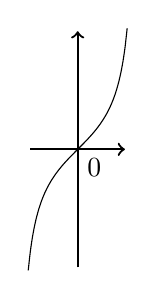
\begin{tikzpicture}[scale=0.5]
\draw[thick,->] (0,-3) -- (0,3);
\draw[thick,->] (-1.2,0) -- (1.2,0);
\draw plot[smooth,domain=0:pi/2.5] (\x,{tan(\x r)});
\draw plot[smooth,domain=0:-pi/2.5] (\x,{-tan(-\x r)});
\node at (0,0) [below right] {$0$};
\end{tikzpicture}
\Img{MA2-22.04.2009-IMG-4}

\section{23.04.2009}
\subsection{MA2-23.04.2009-IMG-1}
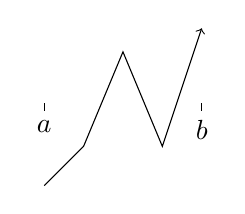
\begin{tikzpicture}
\tikzcoor[x][]{3.5}{1.5}

\foreach \x/\y in{1/a,3/b}
	\draw (\x,-0.05) node[below] {$\y$} -- (\x,0.05);

\draw[->] (1,-1) -- (1.5,-0.5) -- (2, 0.7) -- (2.5,-0.5) -- (3,1);
\end{tikzpicture}
\Img{MA2-23.04.2009-IMG-1}

\subsection{MA2-23.04.2009-IMG-2}
\begin{tikzpicture}

\draw (0.5,0) node[left] {$1 \delta$} -- (3.5,0);
\draw[*-*] (1,-1) -- (1.5,-0.5) -- (2, 0.7) -- (2.5,-0.5) -- (3,1);
\draw (1,-1.5) node[below] {$a$} -- (1,1.5);
\draw (3,-1.5) node[below] {$b$} -- (3,1.5);
\end{tikzpicture}
\Img{MA2-23.04.2009-IMG-2}

\subsection{MA2-23.04.2009-IMG-3}
\begin{tikzpicture}
\tikzcoor[][]{2}{2}

\foreach \x in{0,1}
	\draw[thick] (\x,-0.05) node[below] {$\x$} -- (\x,0.05);

\draw plot[smooth, domain=0.15:2] (\x,{1/\x * 0.3});

\end{tikzpicture}
\Img{MA2-23.04.2009-IMG-3}

\subsection{MA2-23.04.2009-IMG-4}
\begin{tikzpicture}[scale=0.5]
\tikzcoor[][]{12.566}{1.5}
\draw[thick] (0,-1.5) -- (0,1.5);

\draw[thick] (6.283,-0.05) node[below] {$\frac{\pi}{2}$} -- (6.283,0.05);

\draw plot[smooth, domain=0:12.566] (\x,{sin(\x r)});

\end{tikzpicture}
\Img{MA2-23.04.2009-IMG-4}

\subsection{MA2-23.04.2009-IMG-5}
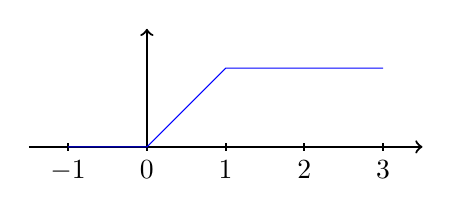
\begin{tikzpicture}
\draw[thick, ->] (-1.5,0) -- (3.5,0);
\draw[thick, ->] (0,0) -- (0,1.5);

\foreach \x in {-1,0,...,3}
	\draw[thick] (\x,-0.05) node[below] {$\x$} -- (\x,0.05);

\draw[blue] (-1,0) -- (0,0) -- (1,1) -- (2,1) -- (3,1);
\end{tikzpicture}
\Img{MA2-23.04.2009-IMG-5}

\section{28.04.2009}
\subsection{MA2-28.04.2009-IMG-1}
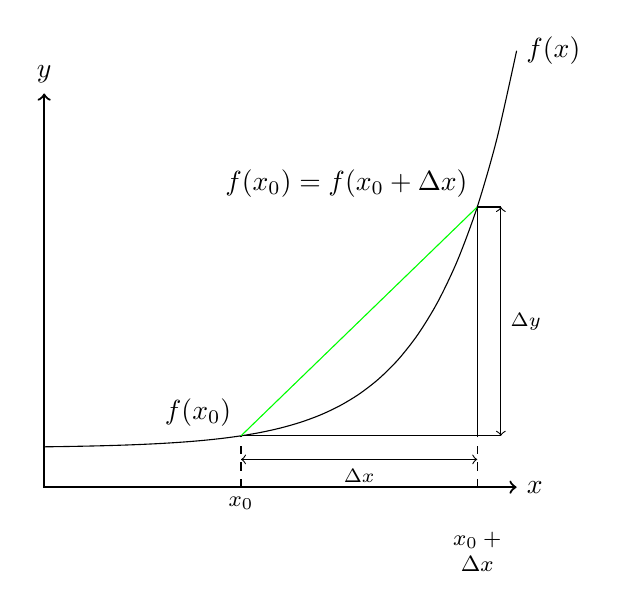
\begin{tikzpicture}[domain=0:6]
\draw[<->,thick] (0,5) node[above] {$y$} -- (0,0) -- (6,0) node[right] {$x$};
\draw plot[smooth] (\x,{exp(\x)/80 + 0.5}) node[right] {$f(x)$};
\draw (2.5,{exp(2.5)/80 + 0.5}) -- (5.5,{exp(2.5)/80 + 0.5}) -- (5.5,{exp(5.5)/80 + 0.5});
\draw[color=green] (2.5,{exp(2.5)/80 + 0.5}) node[above left, color=black] {$f(x_0)$} -- (5.5,{exp(5.5)/80 + 0.5}) node[above left, color=black] {$f(x_0) = f(x_0 + \Delta x)$};
\draw[dashed] (2.5,0) node[below] {\footnotesize{$x_0$}} -- (2.5,{exp(2.5)/80 + 0.5});
\draw[dashed] (5.5,0) node[below, text width=7mm] {\begin{center}\footnotesize{$x_0 + \Delta x$}\end{center}} -- (5.5,{exp(5.5)/80 + 0.5});

\draw[<->] (2.5,{exp(2.5)/80 + 0.2}) -- (5.5,{exp(2.5)/80 + 0.2}) node[below, midway] {\scriptsize{$\Delta x$}};
\draw (5.5,{exp(2.5)/80 + 0.5}) -- (5.8,{exp(2.5)/80 + 0.5});
\draw (5.5,{exp(5.5)/80 + 0.5}) -- (5.8,{exp(5.5)/80 + 0.5});
\draw[<->] (5.8,{exp(2.5)/80 + 0.5}) -- (5.8,{exp(5.5)/80 + 0.5}) node[right, midway] {\scriptsize{$\Delta y$}};
\end{tikzpicture}
\Img{MA2-28.04.2009-IMG-1}
